\documentclass[10pt,journal,compsoc]{IEEEtran}
\usepackage{cite}
\usepackage{amsmath,amssymb,amsfonts}
\usepackage{mathtools}
\usepackage{graphicx}
\usepackage[table]{xcolor}
\usepackage{booktabs}
\usepackage{multirow}
\usepackage{siunitx}
\usepackage[hidelinks]{hyperref}
\usepackage{tikz}
\usetikzlibrary{arrows.meta,positioning,shapes,fit,calc}
\usepackage{caption}
\usepackage{subcaption}
\usepackage{enumitem}
\usepackage{balance} % final column balance

% Compact spacing
\setlength{\abovecaptionskip}{4pt}
\setlength{\belowcaptionskip}{6pt}
\setlength{\textfloatsep}{8pt}
\setlength{\floatsep}{6pt}
\setlist{noitemsep,leftmargin=*}

% Title and author
\title{A Decentralized Screenless Mobile: Mesh-First Connectivity, DTN Resilience, and Self-Sovereign Identity}
\author{Rohit Rajat%
\thanks{Email: \texttt{it.2003138@gmail.com}}%
}

\begin{document}
\maketitle
% Uncomment and edit the following line for journal header if required:
% \markboth{Journal Name,~Vol.~X, No.~X, Month~Year}{}

\begin{abstract}
This paper presents the design of a decentralized, screenless mobile device that prioritizes proximity mesh links (Wi-Fi Aware/NAN), efficient voice transport (Bluetooth LE Audio/LC3), and long-range, low-power links (LoRa) with Delay/Disruption-Tolerant Networking (DTN) for store-and-forward, secured end-to-end with decentralized identifiers (DIDs) and Matrix-style cryptography. Inspired by mesh telephony deployments (Serval, Village Telco) and recent screenless assistants, the architecture addresses usability and resilience via local-first design, E2E encryption, and opportunistic federation. We detail hardware/software stack, interaction model, security, energy considerations, and an evaluation plan, and include implementable diagrams suitable for IEEE figures.
\end{abstract}

\begin{IEEEkeywords}
Decentralized mobile, mesh telephony, Wi-Fi Aware, LE Audio LC3, LoRa, DTN, DIDs, Matrix, wearable HCI.
\end{IEEEkeywords}

\section{Introduction}
Screenless wearables illustrate the promise of voice-first mobility and the pitfalls of cloud dependence, motivating a local-first, decentralized rethink of the ``phone'' without a display. Community mesh telephony projects (Serval, Village Telco) demonstrated infrastructure-free calling and messaging in disasters and underserved regions using ad-hoc Wi-Fi and mesh relays. DTN and decentralized identity complete the resilience and trust story by enabling eventual delivery across disruptions and portable authentication without centralized accounts.

\section{Background and Related Work}
\subsection{Mesh telephony and Serval / Village Telco}
Serval integrated device-to-device calling over Wi-Fi with store-and-forward (Rhizome) and mesh extenders. Village Telco validated VoIP over community WLAN mesh with satisfactory QoS and adoption metrics.

\subsection{Delay/Disruption-Tolerant Networking (DTN)}
DTN's Bundle Protocol decouples endpoints in space and time and supports store-and-forward across intermittent links.

\subsection{Decentralized Identity and Matrix}
W3C DIDs enable self-sovereign identifiers and verifiable credentials; Matrix provides decentralized, federated, end-to-end encrypted messaging suited for opportunistic federation when IP is available.

\section{System Goals}
The system goals are:
\begin{itemize}
  \item Connectivity independent of infrastructure (mesh first).
  \item Graceful degradation under disruption (DTN store-and-forward).
  \item Privacy-preserving identity and messaging without centralized accounts (DIDs + Matrix).
  \item Audio/haptic-first interaction (LE Audio/LC3 for low bitrate voice).
  \item Modular radios and low energy footprint by omitting a display.
\end{itemize}

\section{System Architecture}
\subsection{Hardware}
An always-on low-power MCU handles wake-word and sensor gating; an application SoC runs networking and inference. Audio I/O includes far-field microphones and speaker or bone conduction; haptics provide private feedback. Radios: Wi-Fi Aware (NAN), BLE (LE Audio / LC3), and LoRa for sparse backhaul.

\subsection{Software and Protocol Stack}
Proximity discovery uses Wi-Fi Aware/NAN; when IP is present Matrix-style E2E messaging is used; DTN bundles provide store-and-forward spanning LoRa and other intermittent links. Identity and authentication rely on DIDs with signed DID Documents.

% -------------------------
% Improved Figure 1: System Block Diagram
% -------------------------
\begin{figure}[!t]
\centering
\resizebox{0.95\columnwidth}{!}{%
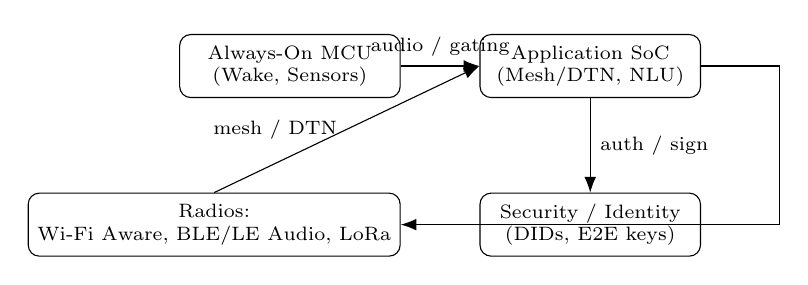
\begin{tikzpicture}[font=\scriptsize,node distance=12mm and 10mm]
  % Node style
  \tikzstyle{comp}=[draw,rounded corners,minimum width=2.8cm,minimum height=0.8cm,align=center,fill=white]

  % Nodes
  \node[comp] (mcu) {Always-On MCU\\(Wake, Sensors)};
  \node[comp,right=of mcu] (soc) {Application SoC\\(Mesh/DTN, NLU)};
  \node[comp,below=of soc] (sec) {Security / Identity\\(DIDs, E2E keys)};
  \node[comp,left=of sec] (radios) {Radios:\\Wi-Fi Aware, BLE/LE Audio, LoRa};

  % Connections with adjusted label positions
  \draw[-{Latex[length=2mm]}] (mcu.east) -- (soc.west) node[pos=0.5,above]{audio / gating};
  \draw[-{Latex[length=2mm]}] (soc.south) -- (sec.north) node[pos=0.5,right]{auth / sign};
  \draw[-{Latex[length=2mm]}] (radios.north) -- (soc.west) node[pos=0.5,left]{mesh / DTN};
  \draw[-{Latex[length=2mm]}] (soc.east) -- ++(10mm,0) |- (radios.east);
\end{tikzpicture}%
}
\caption{System block diagram (compact, improved layout to prevent overlapping labels).}
\label{fig:block}
\end{figure}

\section{Interaction Model}
The device is voice/haptics-first: wake-word, spoken confirmations, and tactile cues. LE Audio/LC3 improves intelligibility at low bitrates, lowering airtime and power. Non-visual controls use tactile patterns for discreet notifications and mode switching. Context disambiguation leverages wearable HCI techniques for audio-only outputs.

\section{Security and Privacy}
Identity and trust are anchored in W3C DIDs with signed DID Documents and verifiable credentials; peers verify control and rotate keys without centralized registries. For messaging over IP, Matrix federation with E2E encryption prevents intermediaries from reading content while allowing self-hosted homeservers. Hardware privacy controls include physical mic mute and capture-LED transparency.

% -------------------------
% Improved Figure 2: Protocol Stack
% -------------------------
\begin{figure}[!t]
\centering
\resizebox{0.85\columnwidth}{!}{%
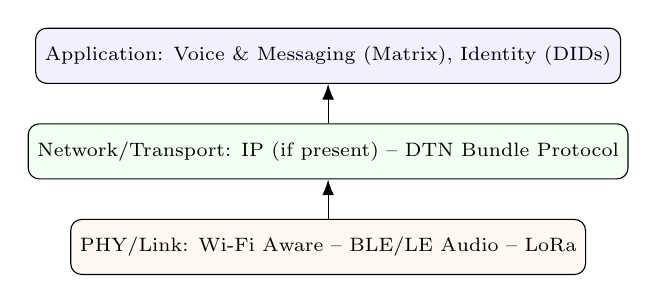
\begin{tikzpicture}[font=\scriptsize, node distance=3mm]
  % Layers as boxes
  \node[draw,rounded corners,fill=blue!6,minimum width=6.5cm,minimum height=0.7cm] (app) {Application: Voice \& Messaging (Matrix), Identity (DIDs)};
  \node[draw,rounded corners,fill=green!6,minimum width=6.5cm,minimum height=0.7cm,below=5mm of app] (net) {Network/Transport: IP (if present) -- DTN Bundle Protocol};
  \node[draw,rounded corners,fill=orange!6,minimum width=6.5cm,minimum height=0.7cm,below=5mm of net] (phy) {PHY/Link: Wi-Fi Aware -- BLE/LE Audio -- LoRa};

  % Arrows
  \draw[-{Latex[length=2mm]}] (phy.north) -- (net.south);
  \draw[-{Latex[length=2mm]}] (net.north) -- (app.south);
\end{tikzpicture}%
}
\caption{Protocol stack diagram (improved spacing and readability).}
\label{fig:stack}
\end{figure}

\section{Mode State Machine}
Prefer mesh (Wi-Fi Aware) for discovery and low-latency sessions; use federated IP via Matrix when reachable; fall back to DTN bundles over LoRa and queue for recontact. Reconciliation happens on recontact.

% Figure 3: mode state machine (compact)
\begin{figure}[!t]
\centering
\resizebox{0.95\columnwidth}{!}{%
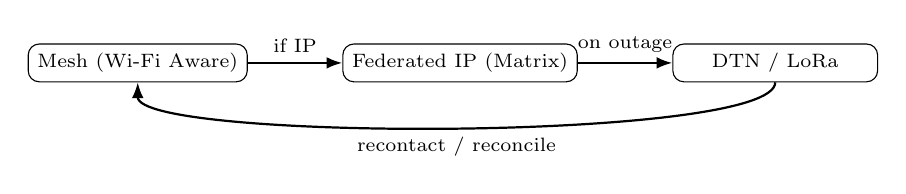
\begin{tikzpicture}[font=\scriptsize, node distance=8mm]
  \node[draw,rounded corners,fill=white,minimum width=2.6cm] (mesh) {Mesh (Wi-Fi Aware)};
  \node[draw,rounded corners,fill=white,minimum width=2.6cm,right=12mm of mesh] (ip) {Federated IP (Matrix)};
  \node[draw,rounded corners,fill=white,minimum width=2.6cm,right=12mm of ip] (dtn) {DTN / LoRa};

  \draw[-{Latex[length=2mm]},thick] (mesh) -- (ip) node[midway,above]{if IP};
  \draw[-{Latex[length=2mm]},thick] (ip) -- (dtn) node[midway,above]{on outage};
  \draw[-{Latex[length=2mm]},thick] (dtn) .. controls +(down:10mm) and +(down:10mm) .. (mesh) node[midway,below]{recontact / reconcile};
\end{tikzpicture}%
}
\caption{Mode state transitions (compact).}
\label{fig:mode}
\end{figure}

\section{Energy Considerations}
Displays dominate smartphone power in many modes; omitting the display improves endurance. LE Audio/LC3 reduces bitrate for comparable quality and improves packet loss resilience, lowering radio duty cycle. Opportunistic DTN transfers on LoRa shift background sync to ultra-low-throughput windows, with ADR balancing reliability and energy.

\section{Proposed Solutions}
\subsection{Mesh-First Communication}
Default to Wi-Fi Aware proximity sessions for discovery, signalling and data; form clusters that maintain calling/messaging functionality without APs.

\subsection{DTN Store-and-Forward}
Use Bundle Protocol overlay to queue and relay messages and voice snippets across partitions ensuring eventual delivery.

\subsection{Sovereign Identity \& E2E}
Adopt DIDs for authentication and Matrix E2E for confidentiality in federated modes to avoid centralized account dependency.

\section{Implementation Plan}
\textbf{Phase 1:} Android-class prototype using Wi-Fi Aware APIs, BLE/LE Audio and external LoRa for DTN validation.  
\textbf{Phase 2:} Integrate DID libraries and Matrix clients for peer auth, E2E messaging and optional federation.  
\textbf{Phase 3:} Field trials mirroring Serval/Village Telco community meshes and disaster exercises.

\section{Evaluation Methodology}
Connectivity: delivery ratio, time-to-deliver, path diversity under induced disruptions comparing mesh-only, DTN-over-mesh, and federated modes.  
Energy: standby and active power with/without voice sessions; quantify savings from eliminating displays and adopting LC3.  
Usability: task completion, error rates, and subjective workload for voice/haptic tasks.

\section{Limitations}
LoRa’s low rate constrains rich media and mandates prioritization of signaling, text and compressed summaries. Wi-Fi Aware support varies by chipset and OEM. Screenless interactions face discoverability challenges.

\section{Future Work}
On-device speech and compact edge LLMs for offline NLU/NLG; multi-radio policy learning to select among radios based on context; community deployment toolkits and governance models.

\section{Conclusion}
Combining mesh-first Wi-Fi Aware, DTN, and sovereign identity with Matrix E2E and a voice/haptics interaction model enables a decentralized, screenless mobile that preserves privacy, degrades gracefully, and improves energy endurance by omitting the display.

\section*{Acknowledgment}
The authors acknowledge prior community mesh telephony efforts and open standards communities underpinning decentralized connectivity and identity.

% -------------------------
% Bibliography (manual entries compatible with IEEEtran)
% -------------------------
\begin{thebibliography}{99}
\bibitem{wifiaware} Android Developers, ``Wi-Fi Aware overview,'' 2025. [Online]. Available: \url{https://developer.android.com/guide/topics/connectivity/wifiaware}
\bibitem{leaudio} SoundGuys, ``What is LE Audio and LC3,'' 2024. [Online]. Available: \url{https://www.soundguys.com/le-audio-lc3-19934/}
\bibitem{lora} LoRa Alliance, ``LoRaWAN® Specification,'' 2021.
\bibitem{dtn} K. Scott and S. Burleigh, ``Bundle Protocol Specification,'' RFC 5050, Nov. 2007.
\bibitem{dids} W3C, ``Decentralized Identifiers (DIDs) v1.0,'' 2022. [Online]. Available: \url{https://www.w3.org/TR/did-core/}
\bibitem{matrix} Matrix.org Foundation, ``Matrix: an open network for secure, decentralised communication,'' 2024. [Online]. Available: \url{https://matrix.org/docs/guides/introduction}
\bibitem{serval} Serval Project, ``Serval Mesh,'' (project site), accessed 2024.
\bibitem{village} M. J. Smith, A. P. Jardine, and S. R. Smith, ``The Village Telco project: community-owned telephony infrastructure,'' EURASIP JWCN, 2011.
\bibitem{humane} C. Constine, ``Humane AI Pin review,'' The Verge, 2024.
\bibitem{carroll} A. Carroll and G. Heiser, ``An Analysis of Power Consumption in a Smartphone,'' in \textit{Proceedings of USENIX ATC}, 2010.
\bibitem{tactcube} S. K. et al., ``TactCube: An Intelligent Device to 'converse' with Smart Environments,'' \textit{Sensors}, 2022.
\bibitem{haptic} Y. Zhang et al., ``Touch IoT enabled by wireless self-sensing and haptic e-skin,'' \textit{Nature Communications Engineering}, 2022.
\bibitem{gaze} R. Doe et al., ``GazePointAR: Context-Aware Multimodal Voice Assistant,'' \textit{ACM Proc.}, 2024.
\bibitem{mobileai} A. Editor, \textit{Mobile AI: Communication and Mobility After the Smartphone}, Springer, 2025.
\end{thebibliography}

% -------------------------
% Author biography with photo
% -------------------------
\begin{IEEEbiography}[{
\includegraphics[width=1in,height=1.25in,clip,keepaspectratio]{IMGROHIT1 (1).jpg}}]{Rohit Rajat}
Rohit Rajat is a software developer and researcher focused on decentralized systems, mobile edge computing, and human-centered wearable interfaces. He graduated with a degree in Information Technology from Punjab Technical University (PTU) and holds a diploma in Computer Science from Sant Longowal Institute of Engineering and Technology. Rohit completed a 6-month internship in API integration with the MERN stack during college and has 2.2 years of professional experience at SS\&C Fintech Services Pvt. Ltd., where he worked on system integration and cloud-enabled financial services. His research interests include mesh networking, delay/disruption-tolerant networking (DTN), decentralized identity (DIDs), screenless HCI, and the intersection of decentralized AI, blockchain, and quantum computing for resilient systems.
\end{IEEEbiography}

\balance
\end{document}
